\section{Phase 1: Data Acquisition}
\label{sec:phase1_collection}
To train any deep learning model for estimating blood glucose non-invasively, we need a reliable dataset. This dataset must connect raw signals from a smartphone to actual, accurate blood glucose readings. Since there are no clean, publicly available datasets that match smartphone camera readings with real medical measurements, we had to build our own data collection system.

This section explains how we designed a mobile application called \textit{DiabetesCollector} and how our team organized a real-world data collection campaign at the University Hospital to gather data from actual patients.

\subsection{The Data Collection Campaign at University Hospital}
To make sure our project is based on real clinical data, our faculty provided us with certified medical equipment, and we practically implemented our work in a real medical environment.

\subsubsection{Medical Equipment Provided by Faculty}
Our college provided our team with official \textbf{Accu-Chek} capillary blood glucometers along with their chemical test strips and sterile lancets. The Accu-Chek device is widely trusted in hospitals and clinics for its high accuracy, making it the perfect tool to establish our reference target (the ground truth). 

\subsubsection{Hospital Environment and Ethics}
We conducted our data collection campaign inside the \textbf{University Hospital}. This allowed us to interact with a wide variety of people, including healthy individuals and diabetic patients with different blood sugar levels. Before starting any measurement, we followed basic ethical steps:
\begin{itemize}
    \item We introduced ourselves and explained the goal of our graduation project to the participant.
    \item We obtained verbal consent from each patient before taking any measurements.
    \item We followed safety protocols by disinfecting the patient's finger before using the lancet and safely disposing of the medical waste.
\end{itemize}

\subsection{Our Android Application: DiabetesCollector}
To capture the raw optical data from the patient's finger, we developed a custom Android application named \textit{DiabetesCollector}. We designed the app to be fast, simple, and stable so it would not crash or freeze during hospital visits.

\subsubsection{How the App was Built}
\begin{itemize}
    \item \textbf{Programming Language \& UI:} The app is written in \textbf{Kotlin} using \textbf{Jetpack Compose} to create a clean, modern user interface.
    \item \textbf{Architecture (Clean Architecture \& UDF):} We organized the code using Clean Architecture principles. We also used Unidirectional Data Flow (UDF) through a \texttt{ViewModel}. This structure ensures that user actions and UI updates happen in a reliable sequence, preventing data loss while recording.
    \item \textbf{Database (ObjectBox):} Instead of using heavy SQL databases, we integrated \textbf{ObjectBox}, which is a lightweight NoSQL database. It securely saves patient details and session forms on the phone instantly.
\end{itemize}

\subsubsection{Using the Camera (CameraX API)}
The most critical part of the app is the camera controller, which uses the \textbf{Android Jetpack CameraX API}. When the recording starts, the app automatically turns on the phone’s back LED flash (\texttt{Torch Mode}). This shines a strong light through the patient’s finger tissue, allowing the camera sensor to view the blood volume changes beneath the skin (Photoplethysmography or PPG signal).

\subsection{Patient Profiles and Ground Truth Entry}

\subsubsection{Entering Demographic Information}
Before recording any signal, we asked the patient a few simple questions to build their profile in the app. These factors help the deep learning model learn how different bodies affect the signal:
\begin{itemize}
    \item \textbf{Personal Details:} Name, Age, and Biological Gender.
    \item \textbf{Body Metrics:} Height (in cm) and Weight (in kg).
    \item \textbf{Medical History:} Smoking status (Yes/No) and whether they have other chronic health issues.
\end{itemize}

\subsubsection{Logging the Reference Glucose Level}
Right before or after recording the finger video, we checked the patient's actual blood sugar using the \textbf{Accu-Chek} glucometer. We then manually typed this exact number (in $mg/dL$) into the application's form, which is structured to capture both historical and clinical metrics seamlessly as shown in Figure~\ref{fig:new_record}. This number acts as the label or "ground truth" that our deep learning model will try to predict.

\begin{figure}[H]
    \centering
    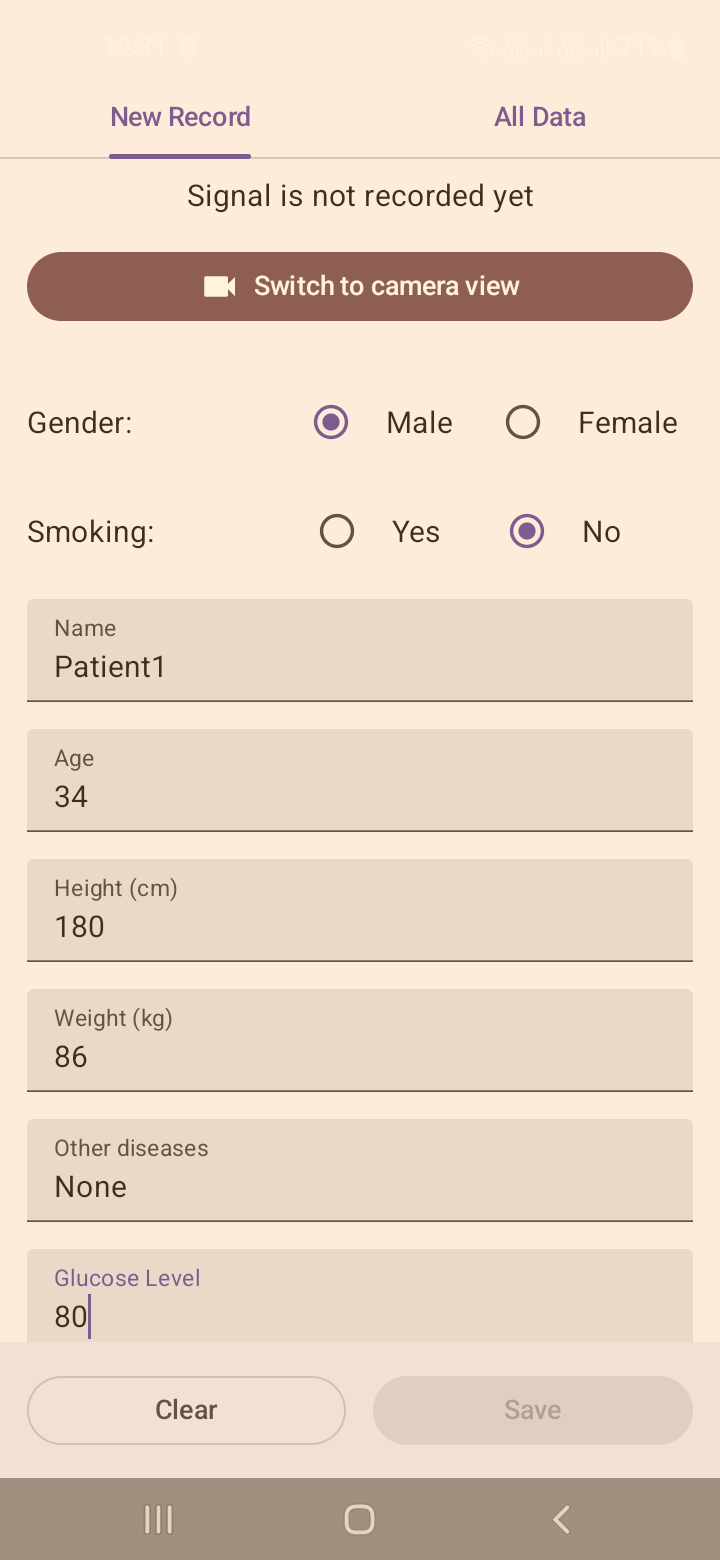
\includegraphics[width=0.45\textwidth]{figures/chapter3/new_record_form.png}
    \caption{The New Record Form interface where patient demographics and Accu-Chek readings are entered.}
    \label{fig:new_record}
\end{figure}

\subsubsection{Tracking Different Phone Hardware}
Since our team members used different smartphones to collect data, the camera sensors were not identical. To handle this, our app automatically reads the phone’s hardware properties from the Android operating system. It saves the \texttt{brand}, \texttt{model}, and \texttt{manufacturer} with every session, so we can fix any hardware differences later during data preprocessing.

\subsection{Handling Data without Overlaps (UUID Strategy)}
Since multiple team members were gathering data at the hospital using different phones at the same time, we faced a technical challenge: how do we merge all the data into one computer later without mixing up patient IDs?

If we used normal numbers like $1, 2, 3$, Phone A and Phone B would both create a "Patient \#1", causing data corruption during merging. To solve this, we used \textbf{Universally Unique Identifiers (UUID Version 4)}. Every time a session is created, the app generates a unique 128-bit random ID. Because this ID is globally unique, we successfully merged all databases from all phones with zero errors or overlaps.

\subsection{The Signal Recording Process (The 20-Second Rule)}
To get clean data with the highest quality, we followed a strict, step-by-step process for every patient. The participant is asked to sit comfortably and place the tip of their index finger gently over the rear camera lens and flash. They must cover the lens completely without pressing too hard, as excessive pressure blocks capillary blood flow. 

The collector then verifies via the live screen preview that the entire matrix view has turned deep red, indicating proper light transmittance through the vascular tissue. Once validated, the active 20-second countdown recording session is initiated to capture between $20$ to $35$ complete cardiac cycles, providing a stable window for future signal analysis while preventing thermal throttling of the hardware. The user interfaces designed for handling this visual alignment and recording process are shown in Figure~\ref{fig:recording_steps}.

\begin{figure}[H]
    \centering
    \begin{subfigure}[b]{0.45\textwidth}
        \centering
        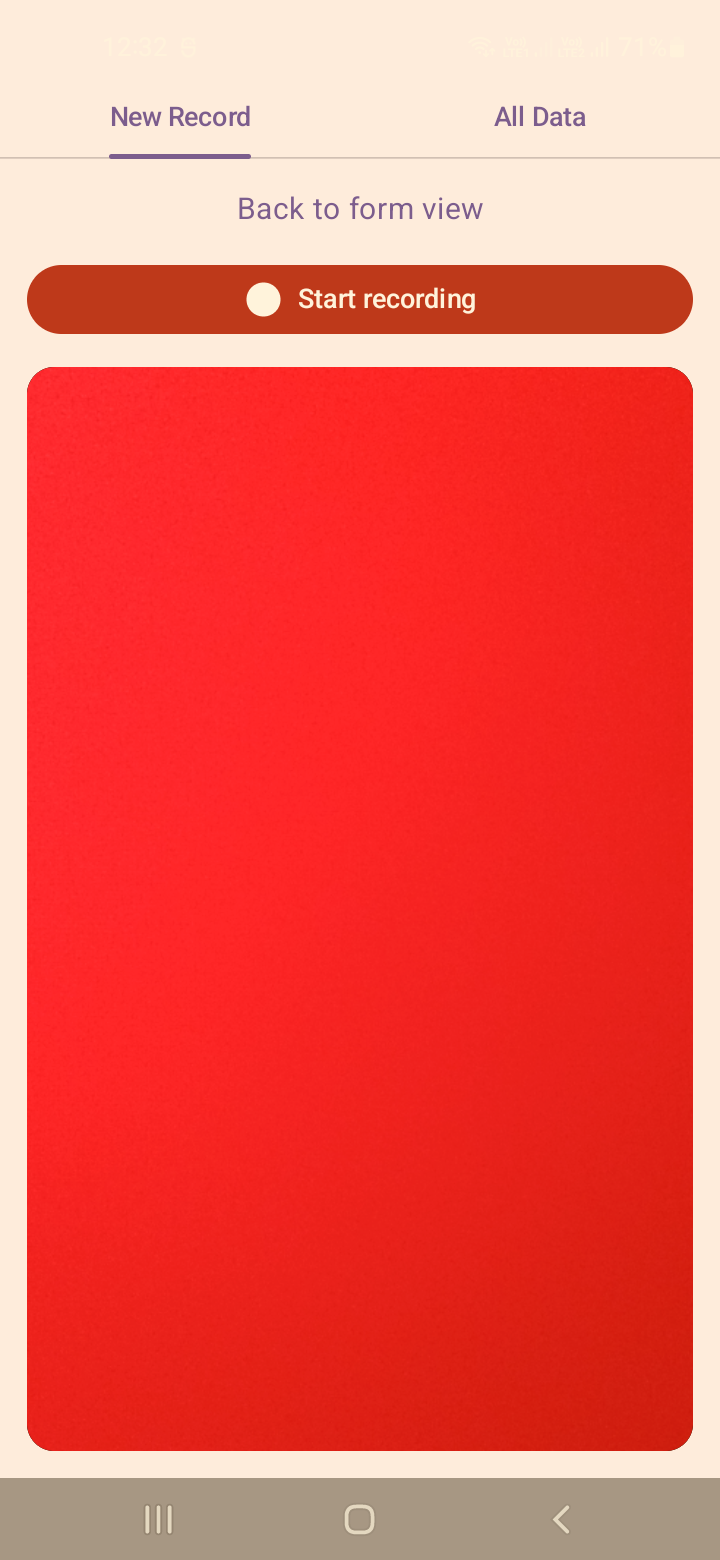
\includegraphics[width=0.9\textwidth]{figures/chapter3/camera_preview.png}
        \caption{Camera Preview Screen}
        \label{subfig:preview}
    \end{subfigure}
    \hfill
    \begin{subfigure}[b]{0.45\textwidth}
        \centering
        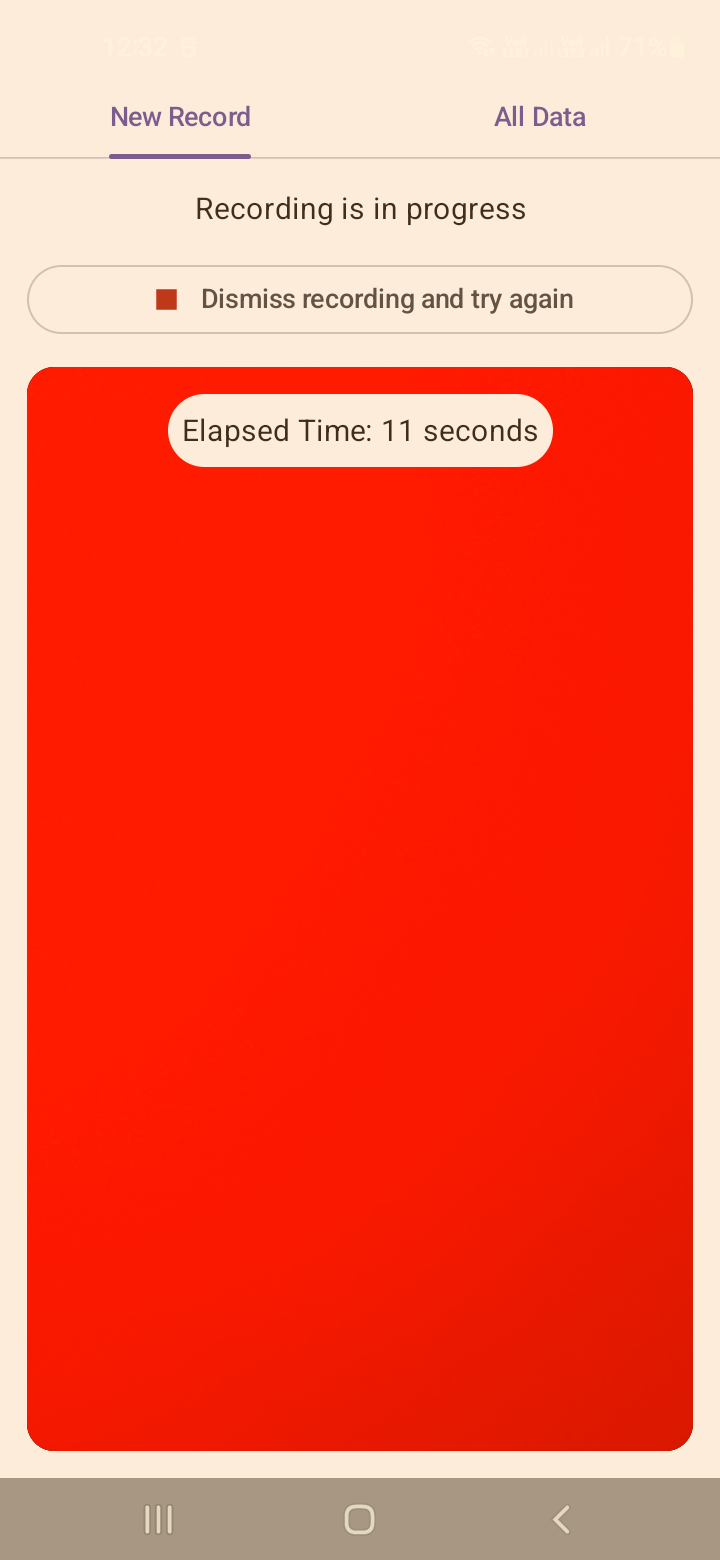
\includegraphics[width=0.9\textwidth]{figures/chapter3/recording_in_progress.png}
        \caption{Active Countdown Recording}
        \label{subfig:recording}
    \end{subfigure}
    \caption{The user interfaces designed for checking the finger alignment and executing the 20-second signal capture sequence.}
    \label{fig:recording_steps}
\end{figure}

\subsection{Exporting and Merging the Final Dataset}

\subsubsection{File Structure on the Phone}
After completing our visits to the University Hospital, we used the built-in export feature in our app. It compresses everything into a single ZIP archive, formatted as: \\
\texttt{diabetes\_collector\_export\_[DATE].zip}. \\
Inside the folder, the raw file components look like this:

\newpage

\begin{verbatim}
diabetes_collector_export_[DATE].zip/
|
|-- patients.csv
|-- video_files/
    |-- uuid_1.mp4
    |-- uuid_2.mp4
    |-- uuid_n.mp4
\end{verbatim}

The application provides intuitive screens to manage this local storage and to trigger the internal zip compression engine, as illustrated in Figure~\ref{fig:management_export}.

\begin{figure}[H]
    \centering
    \begin{subfigure}[b]{0.45\textwidth}
        \centering
        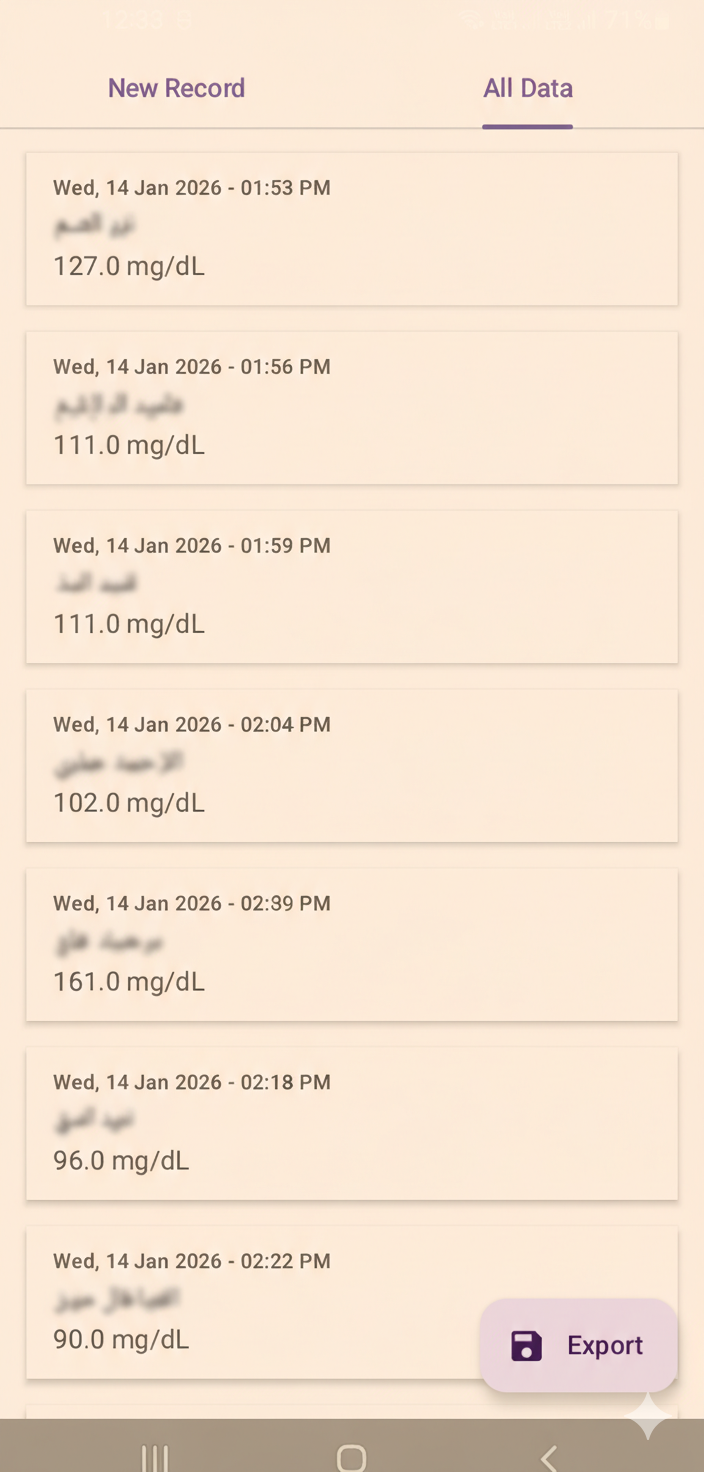
\includegraphics[width=0.9\textwidth]{figures/chapter3/all_data_list.png}
        \caption{Local Database History View}
        \label{subfig:history}
    \end{subfigure}
    \hfill
    \begin{subfigure}[b]{0.45\textwidth}
        \centering
        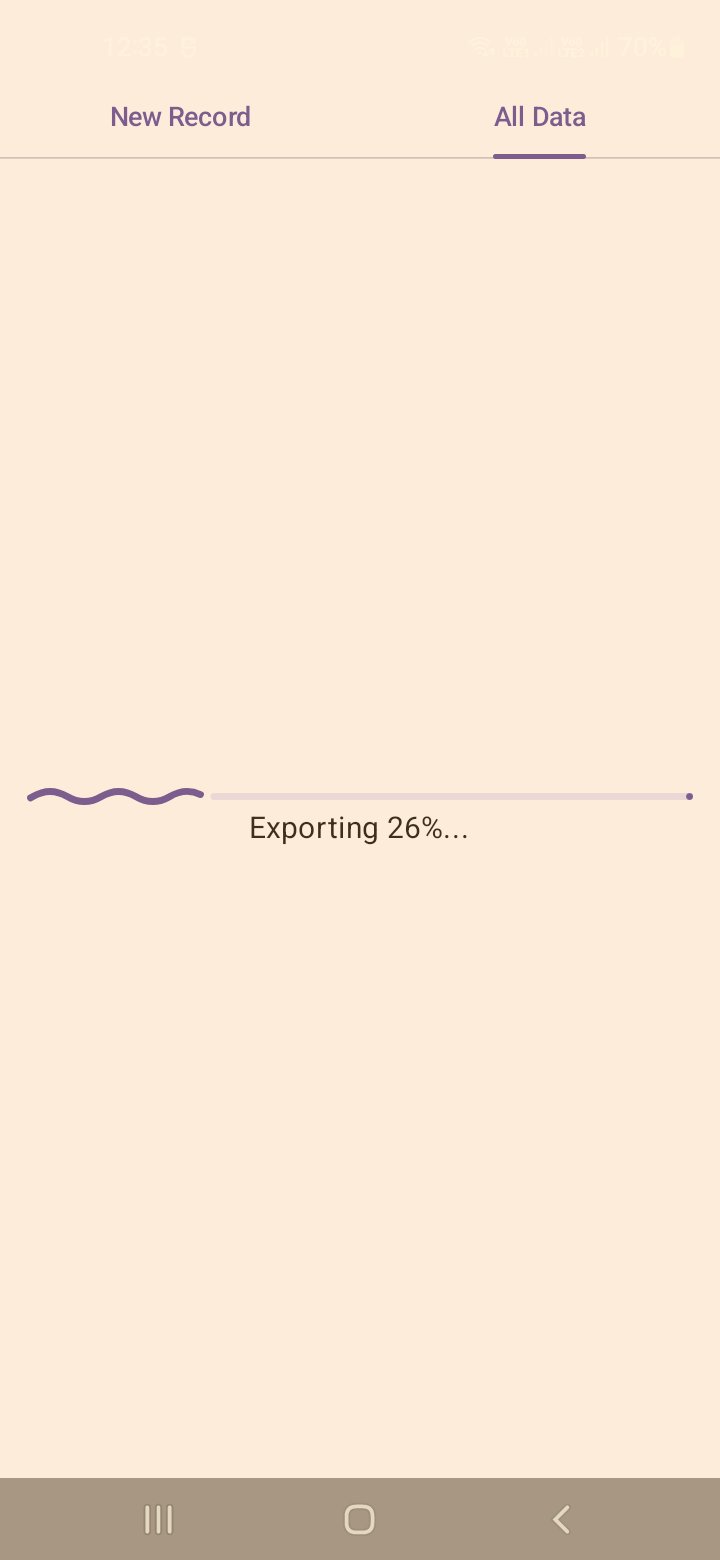
\includegraphics[width=0.9\textwidth]{figures/chapter3/exporting.png}
        \caption{ZIP File Generation Screen}
        \label{subfig:export}
    \end{subfigure}
    \caption{Data management screens showing local storage monitoring and the final data export engine workflow.}
    \label{fig:management_export}
\end{figure}

\subsubsection{The Metadata CSV File}
The \texttt{patients.csv} file is a big table that contains all the text and numbers we entered, linked to the video files using the unique UUIDs. Table~\ref{tab:csv_schema} shows how this data is organized.

\begin{table}[H]
\centering
\caption{The Structure of the Exported \texttt{patients.csv} File}
\label{tab:csv_schema}
\vspace{0.5em}
\resizebox{\textwidth}{!}{
\begin{tabular}{|l|l|l|}
\hline
\textbf{Field Name} & \textbf{Data Type} & \textbf{Description / What it Stores} \\ \hline
\texttt{uuid} & String & Unique ID generated for this session. \\ \hline
\texttt{name} & String & Name or initials of the participant. \\ \hline
\texttt{created\_at} & Timestamp & Date and time of the recording. \\ \hline
\texttt{video\_file} & String & The name of the matching \texttt{.mp4} video. \\ \hline
\texttt{age} & Integer & Age of the patient in years. \\ \hline
\texttt{gender} & Categorical & Male or Female. \\ \hline
\texttt{is\_smoking} & Boolean & True if they smoke, False if not. \\ \hline
\texttt{height} & Float & Height of the patient in cm. \\ \hline
\texttt{weight} & Float & Weight of the patient in kg. \\ \hline
\texttt{other\_diseases} & String & Any other chronic illnesses. \\ \hline
\texttt{glucose\_level} & Float & Accu-Chek reading in mg/dL. \\ \hline
\texttt{device} & String & Internal Android device code. \\ \hline
\texttt{brand} & String & Phone brand (e.g., Samsung, Xiaomi). \\ \hline
\texttt{model} & String & Specific model number of the phone. \\ \hline
\texttt{manufacturer} & String & Company that made the phone. \\ \hline
\hline
\end{tabular}
}
\end{table}

\subsubsection{Final Dataset Aggregation}
At the end of the campaign, all team members moved their ZIP files to a central computer. Thanks to the UUID system, we used a short Python script to quickly combine all the CSV files and video folders into one final, large master dataset. This clean dataset is what we used to train and test our deep learning networks in the next phases of the project.
